% !TeX root = ../main.tex
% ============================================================================
% TEMA 1. FUNCIONES DE VARIAS VARIABLES
% ============================================================================
% Archivo secundario de la presentación Beamer.
% Compilar desde la raíz del repositorio (main.tex) o mediante subfiles.
%
% Convenciones de edición:
%   - Cada idea o conclusión se presenta mediante \item.
%   - Las ecuaciones acompañan a la idea correspondiente, sin viñeta propia.
%   - Las imágenes pendientes se mantienen como marcadores de posición.
%   - \figura y \portadatema son comandos definidos en el documento principal.
% ============================================================================

\documentclass[main.tex]{subfiles}

\begin{document}
\graphicspath{{imagenes/tema1/}{../imagenes/tema1/}}

% ----------------------------------------------------------------------------
% PORTADA
% ----------------------------------------------------------------------------
\portadatema{1}{Funciones de varias variables}

% ----------------------------------------------------------------------------
% 1. MOTIVACIÓN Y CONCEPTOS BÁSICOS
% ----------------------------------------------------------------------------
\begin{frame}{¿Para qué sirven en Ingeniería Informática?}
  \vspace*{-6mm}
  \begin{columns}[T,onlytextwidth]
    \begin{column}{0.492\textwidth}
      \tarjetacontexto
        {ctxAmarillo}{ctxAmarilloFondo}
        {\imagenpendiente{ctxAmarillo}{Terreno 3D}}
        {Gráficos y videojuegos}
        {La altura de un terreno depende de su posición.}
        {h=f(x,y)}
    \end{column}
    \begin{column}{0.492\textwidth}
      \tarjetacontexto
        {ctxRojo}{ctxRojoFondo}
        {\imagenpendiente{ctxRojo}{Imagen / píxeles}}
        {Procesamiento de imágenes}
        {La intensidad de un píxel depende de sus coordenadas.}
        {I=f(x,y)}
    \end{column}
  \end{columns}

  \vspace{3mm}

  \begin{columns}[T,onlytextwidth]
    \begin{column}{0.492\textwidth}
      \tarjetacontexto
        {ctxAzul}{ctxAzulFondo}
        {\imagenpendiente{ctxAzul}{Modelo de IA}}
        {Inteligencia artificial}
        {Una predicción depende de múltiples características.}
        {\hat y=f(x_1,\ldots,x_n)}
    \end{column}
    \begin{column}{0.492\textwidth}
      \tarjetacontexto
        {ctxVerde}{ctxVerdeFondo}
        {\imagenpendiente{ctxVerde}{Procesadores}}
        {Rendimiento de sistemas}
        {El tiempo depende del tamaño de los datos y del número de procesadores.}
        {T=f(n,p)}
    \end{column}
  \end{columns}
\end{frame}

% Definición de función; ejemplo con una variable.
\begin{frame}{Concepto de función}
  \begin{columns}[c,onlytextwidth]
    \begin{column}{0.54\textwidth}
      \begin{itemize}
        \item Una \textbf{función} es una correspondencia entre un conjunto de
              entrada (\textbf{dominio}) y uno de salida (\textbf{codominio})
              que asigna a cada elemento del dominio un único elemento del
              codominio.

        \item Por ejemplo, para $f(x)=x^2$, podemos expresar
              el valor de salida mediante la variable $y$:
              \[
                y=f(x)=x^2
              \]

        \item La variable $x$ es \textbf{independiente} y la variable $y$
              es \textbf{dependiente}.
      \end{itemize}
    \end{column}
    \begin{column}{0.42\textwidth}
      \centering
      % FIGURA PENDIENTE: parábola y=x^2, ejes y puntos destacados.
      \fbox{\parbox[c][4.8cm][c]{0.9\linewidth}{\centering\small
        Gráfica de la parábola $y=x^2$, con ejes $x$ e $y$, vértice
        en el origen y algunos puntos destacados.
      }}
    \end{column}
  \end{columns}
\end{frame}

% Dominio: función definida en todos los reales.
\begin{frame}{Dominio de una función}
  \begin{columns}[c,onlytextwidth]
    \begin{column}{0.54\textwidth}
      \begin{itemize}
        \item El \textbf{dominio} es el conjunto de valores de la variable
              independiente para los que la función está definida.

        \item Para la función $f(x)=x^2$, cualquier número real
              puede utilizarse como entrada:
              \[
                \operatorname{Dom}(f)=\mathbb{R}
              \]

        \item Por tanto, la función está definida para \textbf{todos los
              números reales}.
      \end{itemize}
    \end{column}
    \begin{column}{0.42\textwidth}
      \centering
      % FIGURA PENDIENTE: extensión de la parábola en ambos sentidos.
      \fbox{\parbox[c][5cm][c]{0.9\linewidth}{\centering\small
        Gráfica de $y=x^2$, destacando que la curva se extiende
        indefinidamente hacia la izquierda y hacia la derecha.
      }}
    \end{column}
  \end{columns}
\end{frame}

% Dominio: función racional con un punto excluido.
\begin{frame}{Dominio de una función}
  \begin{columns}[c,onlytextwidth]
    \begin{column}{0.54\textwidth}
      \begin{itemize}
        \item No todas las funciones están definidas para cualquier
              número real.

        \item Consideremos la función:
              \[
                g(x)=\frac{1}{x-2}
              \]

        \item El denominador no puede ser cero:
              \[
                x-2\neq 0
              \]

        \item Su dominio contiene todos los números reales
              \textbf{excepto $x=2$}:
              \[
                \operatorname{Dom}(g)=\mathbb{R}\setminus\{2\}
              \]
      \end{itemize}
    \end{column}
    \begin{column}{0.42\textwidth}
      \centering
      % FIGURA PENDIENTE: dos ramas y asíntota vertical x=2.
      \fbox{\parbox[c][5cm][c]{0.9\linewidth}{\centering\small
        Gráfica de $y=1/(x-2)$, con sus dos ramas y la asíntota vertical
        $x=2$ indicada mediante una línea discontinua.
      }}
    \end{column}
  \end{columns}
\end{frame}

% Diferencia entre codominio e imagen.
\begin{frame}{Codominio e imagen de una función}
  \begin{columns}[c,onlytextwidth]
    \begin{column}{0.54\textwidth}
      \begin{itemize}
        \item El \textbf{codominio} es el conjunto declarado para los
              posibles valores de salida de la función.

        \item La \textbf{imagen} es el conjunto de valores que la función
              alcanza realmente.

        \item Por ejemplo, para la función $f(x)=x^2$ declarada como
              $f:\mathbb{R}\longrightarrow\mathbb{R}$, el codominio
              y la imagen difieren porque $x^2\geq 0$:
              \[
                \begin{aligned}
                  \operatorname{Cod}(f)&=\mathbb{R},\\
                  \operatorname{Im}(f)&=[0,+\infty).
                \end{aligned}
              \]
      \end{itemize}
    \end{column}
    \begin{column}{0.42\textwidth}
      \centering
      % FIGURA PENDIENTE: imagen de la parábola en el eje vertical.
      \fbox{\parbox[c][5cm][c]{0.9\linewidth}{\centering\small
        Gráfica de $y=x^2$, con el eje $y$ resaltado desde $0$ hasta
        $+\infty$ para indicar la imagen de la función.
      }}
    \end{column}
  \end{columns}
\end{frame}

% Ejemplo: codominio e imagen no coinciden.
\begin{frame}{Codominio e imagen de una función}
  \begin{columns}[c,onlytextwidth]
    \begin{column}{0.54\textwidth}
      \begin{itemize}
        \item El dominio y el codominio pueden ser conjuntos distintos,
              y la imagen no tiene por qué coincidir con el codominio.

        \item Consideremos la función:
              \[
                g:\mathbb{R}\setminus\{2\}\longrightarrow\mathbb{R}
              \]
              \[
                g(x)=\frac{1}{x-2}
              \]

        \item Su codominio es $\mathbb{R}$, pero la función nunca toma
              el valor cero:
              \[
                \operatorname{Cod}(g)=\mathbb{R}
              \]
              \[
                \operatorname{Im}(g)=\mathbb{R}\setminus\{0\}
              \]
      \end{itemize}
    \end{column}
    \begin{column}{0.42\textwidth}
      \centering
      % FIGURA PENDIENTE: correspondencias con 0 fuera de la imagen.
      \fbox{\parbox[c][5cm][c]{0.9\linewidth}{\centering\small
        Diagrama de correspondencias entre dominio y codominio.
        El valor $0$ del codominio no recibe ninguna flecha y no
        pertenece a la imagen.
      }}
    \end{column}
  \end{columns}
\end{frame}

% ----------------------------------------------------------------------------
% 2. FUNCIONES DE DOS, TRES Y N VARIABLES
% ----------------------------------------------------------------------------

% Ejemplo aplicado: altura de un terreno como función de dos variables.
\begin{frame}{Funciones de 2 variables}
  \begin{columns}[c,onlytextwidth]
    \begin{column}{0.54\textwidth}
      \begin{itemize}
        \item En Ingeniería Informática, una función de dos variables puede
              modelar la \textbf{altura de un terreno virtual}.

        \item A cada posición $(x,y)$ del mapa le corresponde una
              única altura $h$, que podemos expresar como:
              \[
                h=f(x,y)
              \]

        \item Estas funciones se utilizan para generar escenarios y
              superficies en gráficos por ordenador y videojuegos.
      \end{itemize}
    \end{column}
    \begin{column}{0.42\textwidth}
      \centering
      % FIGURA PENDIENTE: terreno 3D o malla de elevación.
      \fbox{\parbox[c][5cm][c]{0.9\linewidth}{\centering\small
        Terreno 3D o malla de elevación que muestre cómo cada punto
        del plano $(x,y)$ tiene asociada una altura.
      }}
    \end{column}
  \end{columns}
\end{frame}

% Ejemplo aplicado: distancia al origen como función de tres variables.
\begin{frame}{Funciones de 3 variables}
  \begin{columns}[c,onlytextwidth]
    \begin{column}{0.54\textwidth}
      \begin{itemize}
        \item Una función de tres variables puede modelar la
              \textbf{distancia de un objeto al origen} en un entorno 3D.

        \item A cada punto $(x,y,z)$ le corresponde un único
              valor real $d$, dado por:
              \[
                d=f(x,y,z)=\sqrt{x^2+y^2+z^2}
              \]

        \item Estas funciones aparecen en gráficos 3D, simulación,
              realidad virtual y detección de proximidad o colisiones.
      \end{itemize}
    \end{column}
    \begin{column}{0.42\textwidth}
      \centering
      % FIGURA PENDIENTE: ejes 3D, punto y distancia al origen.
      \fbox{\parbox[c][5cm][c]{0.9\linewidth}{\centering\small
        Ejes 3D con un punto $(x,y,z)$ y el segmento desde dicho punto
        hasta el origen, que representa la distancia $d$.
      }}
    \end{column}
  \end{columns}
\end{frame}

% Definición formal de función real de n variables reales.
\begin{frame}{Funciones de varias variables}
  \begin{itemize}
    \item \textbf{Definición:} una función real de $n$ variables reales
          asigna a cada $n$-tupla $(x_1,x_2,\ldots,x_n)$ de su dominio
          un único valor real.
          \[
            f:D\longrightarrow\mathbb{R},\qquad D\subseteq\mathbb{R}^n
          \]
          \[
            u=f(x_1,x_2,\ldots,x_n)
          \]

    \item Los conceptos de \textbf{dominio}, \textbf{codominio}
          e \textbf{imagen} se generalizan directamente a las funciones
          de varias variables.
  \end{itemize}

  % FIGURA PENDIENTE: n entradas, bloque f y una salida.
  \begin{center}
    \fbox{\parbox[c][1.8cm][c]{0.72\linewidth}{\centering\small
      Esquema: varias entradas $(x_1,x_2,\ldots,x_n)$ llegan a un
      bloque $f$, del que sale un único resultado $u$.
    }}
  \end{center}
\end{frame}

% Definición específica de función real de dos variables.
\begin{frame}{Funciones de dos variables}
  \begin{itemize}
    \item Una función real de dos variables asigna a cada par $(x,y)$
          de su dominio $D\subseteq\mathbb{R}^2$ un único valor real:
          \[
            z=f(x,y)
          \]

    \item Las variables $x$ e $y$ son \textbf{independientes} y $z$
          es la \textbf{variable dependiente}.

    \item El \textbf{dominio} contiene los pares $(x,y)$ para los que
          la función está definida; la \textbf{imagen} contiene sus
          valores de salida efectivos.
  \end{itemize}

  % Ilustración existente: entradas y salida de una función de dos variables.
  \figura{s6_0_v2.jpg}{.90}{.30}
\end{frame}

% Representación geométrica: curva frente a superficie.
\begin{frame}{Gráficas de funciones}
  \begin{columns}[c,onlytextwidth]
    \begin{column}{0.68\textwidth}
      \begin{itemize}
        \item \textbf{Funciones de una variable:} la gráfica de
              $y=f(x)$ está formada por puntos $(x,y)$ del plano
              $\mathbb{R}^2$ y es una \textbf{curva}.
              \[
                x\in D\subseteq\mathbb{R}
                \longrightarrow (x,y)\in\mathbb{R}^2
              \]

        \item \textbf{Funciones de dos variables:} la gráfica de
              $z=f(x,y)$ está formada por puntos $(x,y,z)$ del espacio
              $\mathbb{R}^3$ y es una \textbf{superficie}.
              \[
                (x,y)\in D\subseteq\mathbb{R}^2
                \longrightarrow (x,y,z)\in\mathbb{R}^3
              \]
      \end{itemize}
    \end{column}
    \begin{column}{0.29\textwidth}
      \centering
      \figura{s8_2.png}{.90}{.65}
    \end{column}
  \end{columns}
\end{frame}

% Ejemplo de gráfica de una función de dos variables.
\begin{frame}{Funciones de varias variables}
  \begin{itemize}
    \item Consideremos la función de dos variables:
          \[
            z=f(x,y)=x+y^2
          \]

    \item Está definida para cualquier par de números reales:
          \[
            \operatorname{Dom}(f)=\mathbb{R}^2
          \]

    \item Su representación gráfica en el espacio tridimensional
          es una \textbf{superficie}.
  \end{itemize}

  \figura{s9_2.png}{.85}{.43}
\end{frame}

% ----------------------------------------------------------------------------
% 3. CÁLCULO DE DOMINIOS Y OPERACIONES
% ----------------------------------------------------------------------------

% Recordatorio de las restricciones habituales del dominio.
\begin{frame}{Dominios de funciones}
  \footnotesize
  \setbeamerfont{block title}{size=\small}

  \begin{columns}[T,onlytextwidth]
    \begin{column}{0.48\textwidth}
      \begin{block}{Operaciones algebraicas}
        \begin{itemize}
          \item $\displaystyle\frac{1}{A}$: $A\neq 0$.
          \item $\sqrt{A}$: $A\geq 0$.
        \end{itemize}
      \end{block}

      \begin{block}{Funciones logarítmicas}
        \begin{itemize}
          \item $\ln(A)$, $\log(A)$: $A>0$.
        \end{itemize}
      \end{block}

      \begin{block}{Funciones exponenciales}
        \begin{itemize}
          \item $e^x$, $a^x$: dominio $\mathbb{R}$, con $a>0$.
        \end{itemize}
      \end{block}
    \end{column}
    \begin{column}{0.48\textwidth}
      \begin{block}{Funciones trigonométricas}
        \begin{itemize}
          \item $\operatorname{Dom}(\sin)=\operatorname{Dom}(\cos)=\mathbb{R}$.
          \item $\displaystyle\operatorname{Dom}(\tan)
                =\bigl\{x\in\mathbb{R}:x\neq\tfrac{\pi}{2}+k\pi,
                \ k\in\mathbb{Z}\bigr\}$.
        \end{itemize}
      \end{block}

      \begin{block}{Funciones trigonométricas inversas}
        \begin{itemize}
          \item $\operatorname{Dom}(\arcsin)=\operatorname{Dom}(\arccos)
                =[-1,1]$.
          \item $\operatorname{Dom}(\arctan)=\mathbb{R}$.
        \end{itemize}
      \end{block}
    \end{column}
  \end{columns}

  \begin{itemize}
    \item \textbf{Importante:} todas las restricciones deben cumplirse
          simultáneamente.
  \end{itemize}
\end{frame}

% Ejemplo: dominio de una función racional de dos variables.
\begin{frame}{Dominio de funciones de varias variables}
  \begin{columns}[c,onlytextwidth]
    % Columna izquierda: explicación
    \begin{column}{0.6\textwidth}
      \begin{itemize}
        \item \textbf{Ejemplo:} consideremos la función racional:
              \[
                z=f(x,y)=\frac{3x-5y}{y-x^2}
              \]

        \item El denominador no puede ser cero:
              \[
                D=\{(x,y)\in\mathbb{R}^2:y-x^2\neq 0\}
              \]

        \item El dominio es todo $\mathbb{R}^2$ salvo los puntos de la
              parábola $y=x^2$.
      \end{itemize}
    \end{column}

    % Columna derecha: representación gráfica
    \begin{column}{0.4\textwidth}
      \centering
      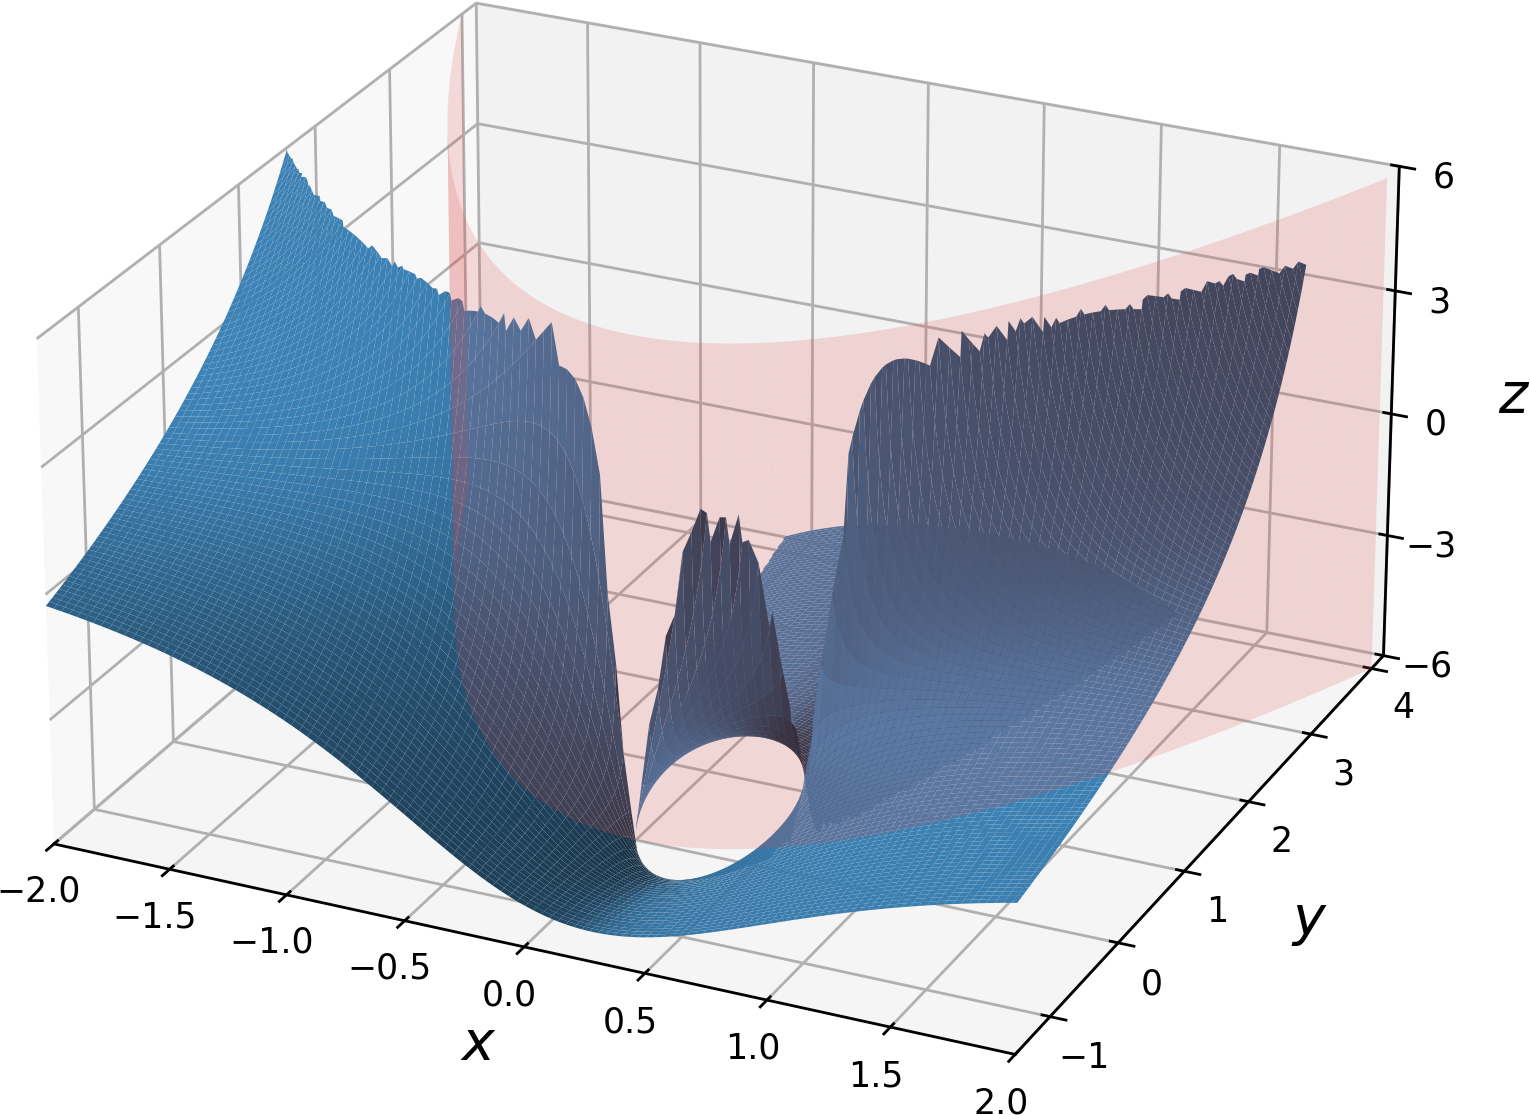
\includegraphics[width=\linewidth]{../python/t01_parabola_domain_sin_margenes.png}
    \end{column}
  \end{columns}
\end{frame}

% Ejemplo: dominio de una raíz cuadrada de dos variables.
\begin{frame}{Dominio de funciones de varias variables}
  \begin{itemize}
    \item \textbf{Ejemplo:} consideremos la función:
          \[
            z=f(x,y)=\sqrt{9-x^2-y^2}
          \]

    \item El radicando debe ser no negativo:
          \[
            D=\{(x,y)\in\mathbb{R}^2:x^2+y^2\leq 9\}
          \]
  \end{itemize}

  \figura{s11_5.png}{.77}{.34}

  \begin{itemize}
    \item El dominio es el \textbf{disco cerrado} de radio $3$ centrado
          en el origen. La gráfica es el hemisferio superior de una esfera.
  \end{itemize}
\end{frame}

% Ejemplo: dominio en R^3 impuesto por un logaritmo.
\begin{frame}{Dominio de funciones de varias variables}
  \begin{columns}[c,onlytextwidth]
    \begin{column}{0.54\textwidth}
      \begin{itemize}
        \item Consideremos la función de tres variables:
              \[
                f(x,y,z)=\ln(z-y)+xy\sin z
              \]

        \item El argumento del logaritmo debe ser positivo:
              \[
                z-y>0
              \]

        \item El dominio es el \textbf{semiespacio} por encima
              del plano $z=y$, sin incluirlo:
              \[
                D=\{(x,y,z)\in\mathbb{R}^3:z>y\}
              \]
      \end{itemize}
    \end{column}
    \begin{column}{0.42\textwidth}
      \centering
      % FIGURA PENDIENTE: plano z=y y semiespacio abierto z>y.
      \fbox{\parbox[c][5cm][c]{0.9\linewidth}{\centering\small
        Representación 3D del plano $z=y$, con el semiespacio $z>y$
        sombreado y el plano frontera excluido del dominio.
      }}
    \end{column}
  \end{columns}
\end{frame}

% Operaciones puntuales entre funciones.
\begin{frame}{Operaciones con funciones de varias variables}
  \begin{itemize}
    \item Las funciones de varias variables admiten \textbf{suma},
          \textbf{producto}, \textbf{cociente} y \textbf{composición},
          siempre que las operaciones estén definidas.

    \item Por ejemplo, la suma de $f(x,y)=x+y$ y $g(x,y)=xy$
          da como resultado:
          \[
            (f+g)(x,y)=x+y+xy
          \]

    \item Las operaciones deben respetar los \textbf{dominios} de las
          funciones implicadas. En particular, los denominadores no
          pueden ser cero.
  \end{itemize}
\end{frame}

% ----------------------------------------------------------------------------
% 4. CURVAS DE NIVEL Y APLICACIONES
% ----------------------------------------------------------------------------

% Definición geométrica de curva de nivel.
\begin{frame}{Curvas de nivel}
  \begin{columns}[c,onlytextwidth]
    % Columna izquierda: explicación
    \begin{column}{0.67\textwidth}
      \begin{itemize}
        \item Las \textbf{curvas de nivel} de una función de dos variables
              están formadas por los puntos $(x,y)$ en los que la función
              toma un mismo valor constante $k$:
              \[
                f(x,y)=k,\qquad k\in\operatorname{Im}(f)
              \]

        \item Se obtienen al intersectar la superficie $z=f(x,y)$ con
              un plano horizontal $z=k$ y proyectar la intersección sobre
              el plano $xy$.
      \end{itemize}
    \end{column}

    % Columna derecha: representación gráfica
    \begin{column}{0.30\textwidth}
      \centering
      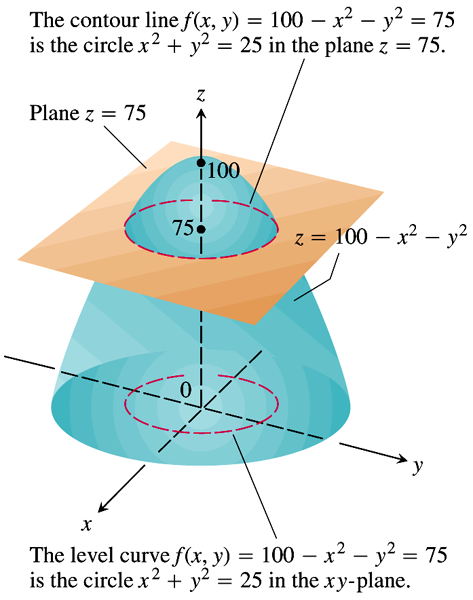
\includegraphics[width=\linewidth]{s14_3.png}
    \end{column}
  \end{columns}
\end{frame}

% Ejemplo resuelto: curvas de nivel de un hemisferio de radio 10.
\begin{frame}{Curvas de nivel}
  \small
  \begin{itemize}
    \item \textbf{Ejemplo:} obtener las curvas de nivel de:
          \[
            z=\sqrt{100-x^2-y^2}
          \]

    \item Fijamos la altura en una constante $z=c$:
          \[
            c=\sqrt{100-x^2-y^2},\qquad c\geq 0
          \]

    \item Elevamos al cuadrado y reorganizamos:
          \[
            c^2=100-x^2-y^2
            \quad\Longrightarrow\quad
            x^2+y^2=100-c^2
          \]

    \item Para $0\leq c<10$ se obtienen \textbf{circunferencias}
          de radio $\sqrt{100-c^2}$. Para $c=10$, solo queda $(0,0)$;
          fuera de $[0,10]$ no hay puntos de nivel.
  \end{itemize}
\end{frame}

% Representación de las circunferencias de nivel.
\begin{frame}{Curvas de nivel}
  \begin{columns}[c,onlytextwidth]
    \begin{column}{0.55\textwidth}
      \begin{itemize}
        \item Consideremos la función:
              \[
                z=\sqrt{100-x^2-y^2}
              \]

        \item Sus curvas de nivel satisfacen:
              \[
                x^2+y^2=100-c^2
              \]

        \item Al aumentar $c$, \textbf{disminuye el radio}
              de las circunferencias.
      \end{itemize}
    \end{column}
    \begin{column}{0.43\textwidth}
      \centering
      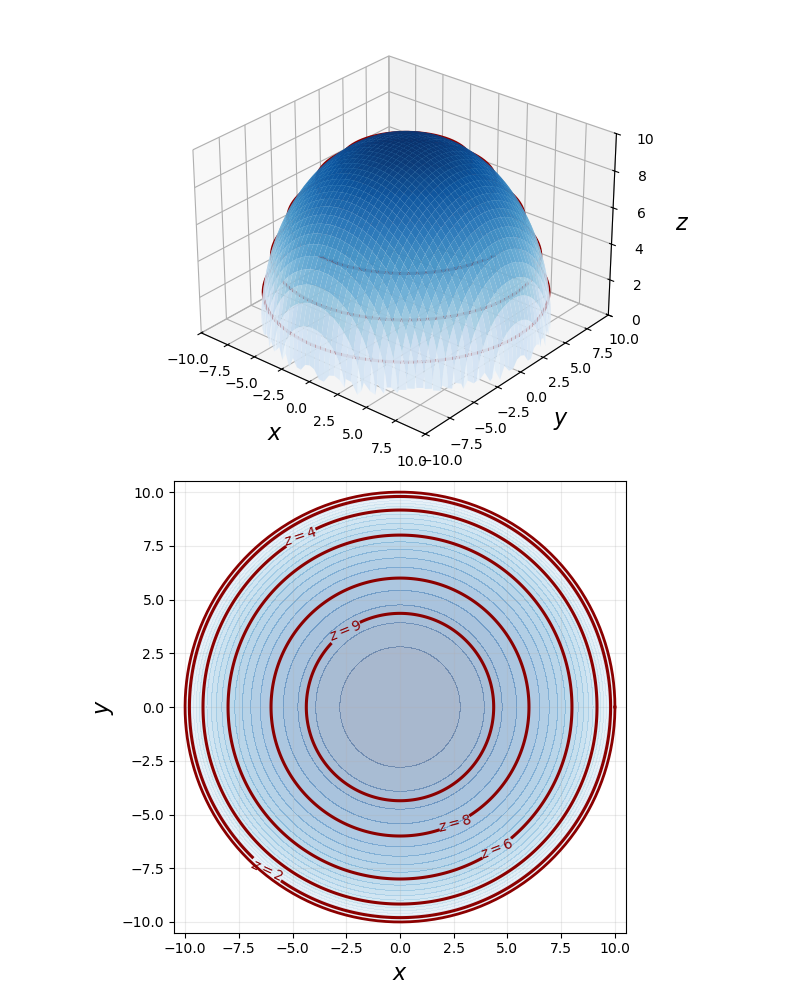
\includegraphics[width=\linewidth]{../python/t01_curvas_nivel_v2.png}
    \end{column}
  \end{columns}
\end{frame}

% Relación entre representación tridimensional y mapa de niveles.
\begin{frame}{Curvas de nivel}
  \begin{itemize}
    \item Una superficie puede representarse mediante sus
          \textbf{curvas de nivel}, que permiten visualizar sus alturas
          sin necesidad de una representación 3D.
  \end{itemize}

  \figura{s18_0.jpg}{.78}{.67}
\end{frame}

% Ejemplo de superficie con valores positivos y negativos.
\begin{frame}{Curvas de nivel}
  \begin{itemize}
    \item Consideremos una función con varios máximos y mínimos:
          \[
            f(x,y)=-xy\,e^{-(x^2+y^2)}
          \]

    \item Sus curvas de nivel permiten identificar las
          \textbf{regiones positivas y negativas} de la superficie.
  \end{itemize}

  \figura{s19_1.jpg}{.97}{.53}
\end{frame}

% Ejemplo de curvas de nivel no circulares.
\begin{frame}{Curvas de nivel}
  \begin{itemize}
    \item Las curvas de nivel pueden tener formas más complejas
          que circunferencias o elipses.

    \item Por ejemplo, consideremos la función:
          \[
            f(x,y)=\frac{-3y}{x^2+y^2+1}
          \]

    \item La figura muestra sus curvas de nivel y la superficie
          tridimensional correspondiente.
  \end{itemize}

  \figura{s20_1.jpg}{.94}{.44}
\end{frame}

% Aplicación de las curvas de nivel a la topografía digital.
\begin{frame}{Curvas de nivel: aplicación topográfica}
  \begin{itemize}
    \item Las curvas de nivel permiten representar la
          \textbf{altura de un terreno} en un mapa bidimensional.

    \item Se utilizan en cartografía digital, sistemas de información
          geográfica y generación de terrenos virtuales en videojuegos.
  \end{itemize}

  \figura{s21_0.jpg}{.68}{.56}
\end{frame}

% ----------------------------------------------------------------------------
% 5. APLICACIÓN INFORMÁTICA: GENERACIÓN DE UNA ESFERA 3D
% ----------------------------------------------------------------------------

% 5.1. Ecuación de la esfera y secciones horizontales.
\begin{frame}{Ejemplo: Generación de una esfera 3D}
  \begin{columns}[c,onlytextwidth]
    \begin{column}{0.59\textwidth}
      \begin{itemize}
        \item En gráficos por ordenador, los objetos 3D pueden
              construirse mediante conjuntos de puntos y superficies.

        \item Queremos generar una \textbf{esfera de radio 1}
              utilizando cinco secciones horizontales.
              Los puntos de la esfera satisfacen:
              \[
                x^2+y^2+z^2=1
              \]

        \item Al fijar una altura $z=k$, cada sección es una
              \textbf{circunferencia}, salvo en los polos, donde
              se reduce a un punto:
              \[
                x^2+y^2=1-k^2
              \]
      \end{itemize}
    \end{column}
    \begin{column}{0.37\textwidth}
      \centering
      % FIGURA PENDIENTE: esfera cortada por cinco planos horizontales.
      \fbox{\parbox[c][5cm][c]{0.9\linewidth}{\centering\small
        Esfera 3D atravesada por cinco planos horizontales que
        muestran sus secciones circulares a distintas alturas.
      }}
    \end{column}
  \end{columns}
\end{frame}

% 5.2. Cálculo del radio de cada sección.
\begin{frame}{Ejemplo: Generación de una esfera 3D}
  \begin{columns}[c,onlytextwidth]
    \begin{column}{0.59\textwidth}
      \begin{itemize}
        \item Seleccionamos cinco alturas:
              \[
                k\in\{-1,-0.5,0,0.5,1\}
              \]

        \item El radio de cada sección se deduce de:
              \[
                x^2+y^2=1-k^2
              \]
              \[
                \rho(k)=\sqrt{1-k^2}
              \]
      \end{itemize}

      % Tabla de valores: es un apoyo numérico, no una idea independiente.
      \[
        \begin{array}{c|c}
          \textbf{Altura }k & \textbf{Radio }\rho \\ \hline
          -1   & 0 \\
          -0.5 & \sqrt{3}/2 \\
          0    & 1 \\
          0.5  & \sqrt{3}/2 \\
          1    & 0
        \end{array}
      \]
    \end{column}
    \begin{column}{0.37\textwidth}
      \centering
      % FIGURA PENDIENTE: secciones etiquetadas por altura y radio.
      \fbox{\parbox[c][5cm][c]{0.9\linewidth}{\centering\small
        Cinco secciones horizontales de una esfera de radio 1,
        etiquetadas con sus alturas $k$ y sus radios $\rho(k)$.
      }}
    \end{column}
  \end{columns}
\end{frame}

% 5.3. Coordenadas cartesianas a partir del ángulo polar.
\begin{frame}{Ejemplo: Generación de una esfera 3D}
  \begin{columns}[c,onlytextwidth]
    \begin{column}{0.59\textwidth}
      \begin{itemize}
        \item Para representar cada sección necesitamos calcular
              puntos de su circunferencia.

        \item Podemos parametrizar sus coordenadas con el ángulo
              $\theta$ y el radio $\rho$:
              \[
                x=\rho\cos\theta,\qquad y=\rho\sin\theta
              \]

        \item Por ejemplo, para $z=0.5$, el radio y las
              coordenadas se obtienen como:
              \[
                \begin{aligned}
                  \rho &= \sqrt{1-0.5^2}=\frac{\sqrt{3}}{2},\\
                  x &= \frac{\sqrt{3}}{2}\cos\theta,\\
                  y &= \frac{\sqrt{3}}{2}\sin\theta.
                \end{aligned}
              \]
      \end{itemize}
    \end{column}
    \begin{column}{0.37\textwidth}
      \centering
      % FIGURA PENDIENTE: sección z=0.5, radio, ángulo y punto.
      \fbox{\parbox[c][5cm][c]{0.9\linewidth}{\centering\small
        Circunferencia horizontal en $z=0.5$, de radio
        $\rho=\sqrt{3}/2$, con un punto $(x,y,0.5)$ indicado
        mediante el ángulo $\theta$.
      }}
    \end{column}
  \end{columns}
\end{frame}

% 5.4. Muestreo angular y construcción de la malla triangular.
\begin{frame}{Ejemplo: Generación de una esfera 3D}
  \small
  \begin{columns}[c,onlytextwidth]
    \begin{column}{0.59\textwidth}
      \begin{itemize}
        \item Seleccionamos \textbf{8 puntos equiespaciados}
              en cada circunferencia:
              \[
                \theta_j=\frac{2\pi j}{8},\qquad j=0,\ldots,7
              \]

        \item En cada altura $z=k$, calculamos las coordenadas:
              \[
                \begin{aligned}
                  x_j &= \rho(k)\cos\theta_j,\\
                  y_j &= \rho(k)\sin\theta_j,\\
                  z_j &= k.
                \end{aligned}
              \]

        \item Los cinco niveles proporcionan \textbf{26 puntos
              distintos}, contando los dos polos.

        \item Al conectar puntos de niveles consecutivos mediante
              triángulos construimos una \textbf{malla 3D} que
              aproxima la esfera.
      \end{itemize}
    \end{column}
    \begin{column}{0.37\textwidth}
      \centering
      % FIGURA PENDIENTE: malla esférica triangulada, 26 vértices.
      \fbox{\parbox[c][5cm][c]{0.9\linewidth}{\centering\small
        Esfera aproximada mediante cinco niveles y 26 vértices
        distintos. Mostrar puntos, polos y conexiones triangulares
        entre secciones.
      }}
    \end{column}
  \end{columns}
\end{frame}

% ----------------------------------------------------------------------------
% MATERIAL ADICIONAL (DESACTIVADO)
% ----------------------------------------------------------------------------
% Se conserva el ejercicio final del borrador original para una posible
% incorporación futura. No aparece en la presentación mientras siga comentado.
%
% \begin{frame}{Funciones de varias variables: ejercicios}
%   \begin{itemize}
%     \item Encontrar el dominio de la función:
%           \[
%             f(x,y,z)=\arcsin(xy)\,e^{3z}+e^{(y+z)\ln(x+z)}
%           \]
%
%     \item Describir los conjuntos de nivel para los valores indicados:
%           \begin{enumerate}[a)]
%             \item $f(x,y)=x^2+y^2$, con $k=0,1,2,3$.
%             \item $f(x,y,z)=x^2+y^2$, con $k=0,1,2$.
%             \item $f(x,y)=x^2-y^2$, con $k=-2,-1,0,1,2$.
%           \end{enumerate}
%
%     \item En a) y c) se obtienen \textbf{curvas de nivel};
%           en b), \textbf{superficies de nivel}.
%   \end{itemize}
% \end{frame}

\end{document}
